\chapter{Sphere collision}
\label{cha:spherecollision}

Spheres are the simplest of bounding shapes used in collision detection. This chapter presents tests for two versions of algorithms -- naive $O(N^2)$ approach and with partitioned space. While the simpler algorithm has a far greater number of collision checks per frame, it allocates almost no memory per frame. A more complex method will minimise the number of checks, but additional structure and steps added may influence overall execution time in an unexpected way.


\begin{figure}[h!]
  \caption{Example rendering of tested sphere collision system}
  \label{img:spheres}
  \centering
	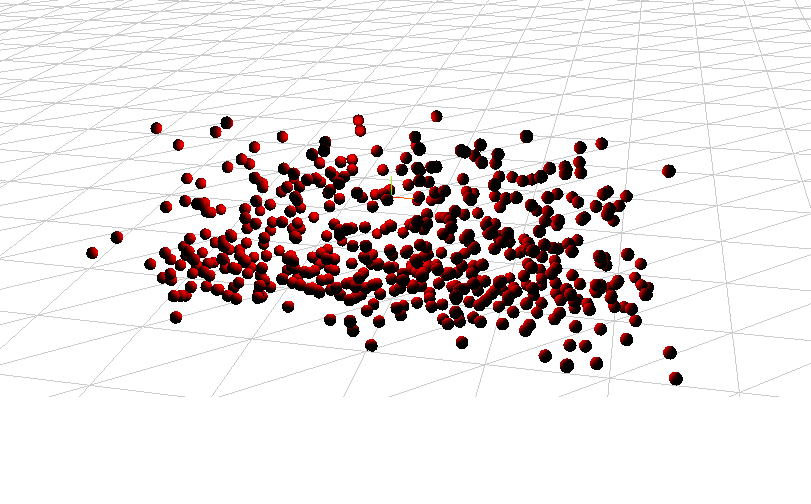
\includegraphics[width=16cm]{spheres/render.png}
\end{figure}

\section{Algorithm description}
\label{sec:spherealgorithmdescription}

Collision detection for spheres is a trivial task. If distance between two spheres is smaller than the sum of their radiuses, spheres collide.

$\sqrt{(S_1.x - S_2.x)^2 + (S_1.y - S_2.y)^2 + (S_1.z - S_2.z)^2} < S_1.radius + S_2.radius$

While the equation is simple, with the large number N of colliding objects the complexity of this detection is $O(N^2)$. Methods of space partitioning are used to reduce the number of checks. The one used in this benchmark is Octree.
The base for the algorithm is a tree-like structure of bounding boxes. Whenever a box contains more than one colliding object, it is divided into eight smaller boxes, by partitioning each edge by 2. When a maximum tree depth is reached, multiple objects are stored in one box. One object may be referenced from multiple boxes, when its size and position make them intersect. Each movement requires a check if the object has already moved to one of the neighbour boxes.

\begin{figure}[h!]
  \caption{Octree structure. Source: http://en.wikipedia.org/wiki/File:Octree2.svg/}
  \label{img:octree2}
  \centering
	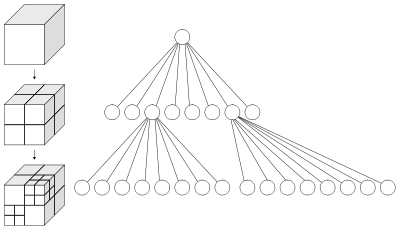
\includegraphics[width=10cm]{octree/octree2.png}
\end{figure} 

Having objects grouped in boxes reduces the complexity of the collision check. Since an object may collide only with objects in the same box, the number of checks is much smaller. Overall complexity of Octree checks is $O(N log{N})$.

\begin{figure}[h!]
  \caption{Example of WebGL Octree debug rendering. Available online at http://pawlowski.it/octtree/}
  \label{img:octree}
  \centering
	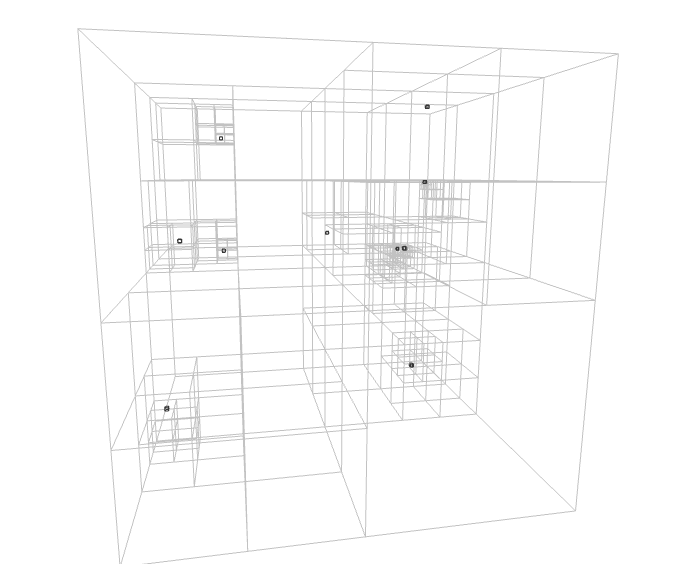
\includegraphics[width=10cm]{octree/octree.png}
\end{figure} 

When collision is detected, collision response is calculated. From the rule of conservation of momentum:

\begin{center}
$m_1 * \vec{v_1} + m_2 * \vec{v_2} = m_1 * \vec{v'_1} + m_2 * \vec{v'_2}$
\end{center}

Meaning that change of both momentums is of equal value.
\begin{center}
$m_1*\vec{v'_1} =  m_1*\vec{v_1} - \Delta P$

$m_2*\vec{v'_2} =  m_2*\vec{v_2} + \Delta P$

$\vec{v'_1} =  \vec{v_1} - \frac{\Delta P}{m_1}$

$\vec{v'_2} =  \vec{v_2} + \frac{\Delta P}{m_2}$
\end{center}

To simplify response, rotation and deformation of spheres are ignored. This does not affect performance analysis, since operations in tests are performed all in the same way.

Let
\begin{center}
$P = |\Delta P|$

$N = \hat{pos_1 - pos_2}$
\end{center}

Since transference of momentum occurs only along single points of contact:
\begin{center}
$ \Delta P = P * \hat{\vec{N}}$

$\vec{v'_1} =  \vec{v_1} - \frac{P}{m_1} * \vec{N}$

$\vec{v'_2} =  \vec{v_2} + \frac{P}{m_2} * \vec{N}$
\end{center}

Let us split each velocity into two scalars, the perpendicular and parallel value of velocity vector, and introduce $\vec{Q}$, similar to $\vec{N}$, a perpendicular normalised vector lining along the exchanged momentum.

 \begin{center}
$\vec{v_1} =  a_1 * \vec{N} + b_1 * \vec{Q}$

$\vec{v_2} =  a_2 * \vec{N} + b_2 * \vec{Q}$

$\vec{v'_1} =  a'_1 * \vec{N} + b'_1 * \vec{Q}$

$\vec{v'_2} =  a'_2 * \vec{N} + b'_2 * \vec{Q}$
\end{center}

\begin{figure}[h!]
  \caption{Illustration for collision response}
  \label{img:spheresbounce}
  \centering
	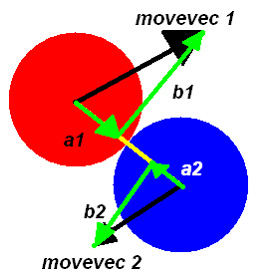
\includegraphics[width=8cm]{spheres/bounce.jpg}
\end{figure} 

Deriving from previous equations:

 \begin{center}
$a_1' =  a_1 - \frac{P}{m_1}$

$b_1' = b_1$

$a_2' =  a_2 + \frac{P}{m_2}$

$b_2' = b_2$
\end{center}

Now let us use the rule of energy conservation to solve P:

 \begin{center}
$\frac{m_1}{2} * ||\vec{v_1}||^2 + \frac{m_2}{2} * ||\vec{v_2}||^2 = \frac{m_1}{2} * ||\vec{v'_1}||^2 + \frac{m_2}{2} * ||\vec{v'_2}||^2$

$\frac{m_1}{2} * ({a_1}^2 + {b_1}^2) + \frac{m_2}{2} * ({a_2}^2 + {b_2}^2) = \frac{m_1}{2} * ({a'_1}^2 + {b'_1}^2) + \frac{m_2}{2} * ({a'_2}^2 + {b'_2}^2)2$

$P = \frac{2*m_1*m_2*(a_1-a_2)}{m_1+m_2}$
\end{center}

and finally, using the result from the conservation of momentum:

 \begin{center}
$\vec{v'_1} =  \vec{v_1} - \frac{2*(a_1-a_2)}{m_1+m_2} * m_2 * \vec{N}$

$\vec{v'_2} =  \vec{v_2} + \frac{2*(a_1-a_2)}{m_1+m_2} * m_1 * \vec{N}$
\end{center}

From this result, using only the dot product of velocity vectors and normalised vector $pos_1 - pos_2$ the correct response to collision is calculated. In tested scenarios, the mass of all spheres is equal since it does not affect the complexity of calculations and produces less random results.


\section{{$O(N^2)$} approach}
\label{sec:sphereinitial}

The naive approach for collision detection proves to by easy to implement in JavaScript. Since almost no memory is allocated in each frame, no garbage collection issues appear. All methods are well defined and work mostly on floats. This results in a highly optimised binary code produced by the compiler, as shown on \ref{img:spheres1profile}.

\begin{figure}[h!]
  \caption{Chart of time used in optimised version of JavaScript}
  \label{img:spheres1profile}
  \centering
	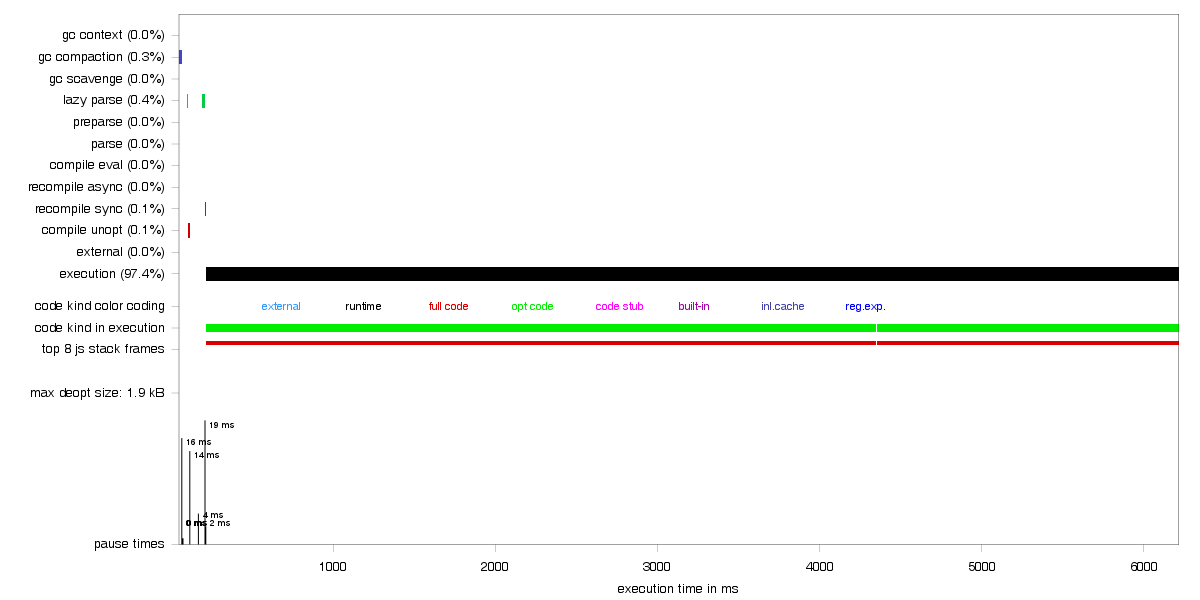
\includegraphics[width=16cm]{spheres/spheres1-profile.png}
\end{figure} 

Multiple tests with N=1000 and different number of frames rendered show that for simple mathematical tasks, the performance of JavaScript is very close to that of C++. On average, the JavaScript version of benchmark runs 15\% longer than a C++ one.

\begin{figure}[h!]
  \caption{Comparison of total execution time. N = 1000, varying number of frames.}
  \label{img:spheres1-time-total}
  \centering
	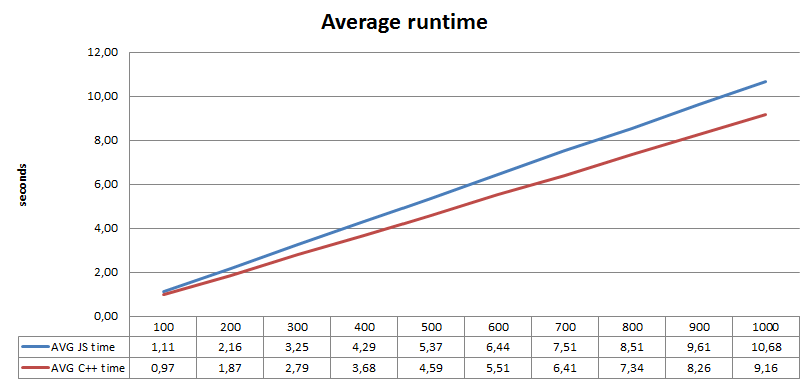
\includegraphics[width=16cm]{spheres/time-total.png}
\end{figure} 
\begin{figure}[h!]
  \caption{Comparison of execution time per frame. N = 1000, varying number of frames.}
  \label{img:spheres1-time-per-frame}
  \centering
	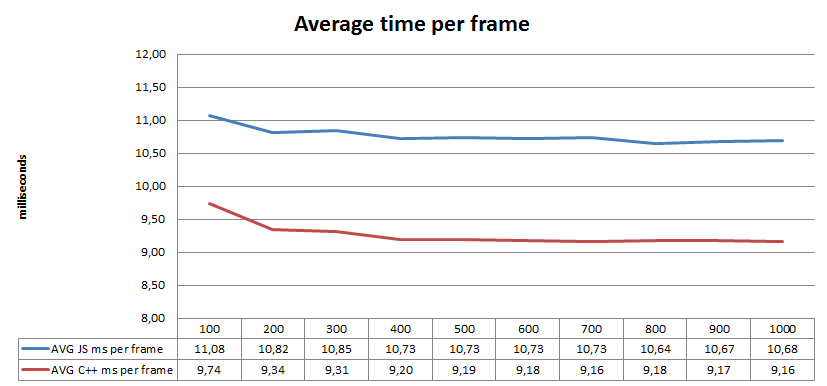
\includegraphics[width=16cm]{spheres/time-per-frame.png}
\end{figure}

\section{Octree-partitioned space}
\label{sec:sphereoctree}

\begin{figure}[h!]
  \caption{Octree partitioned sphere collision system}
  \label{img:spheres}
  \centering
	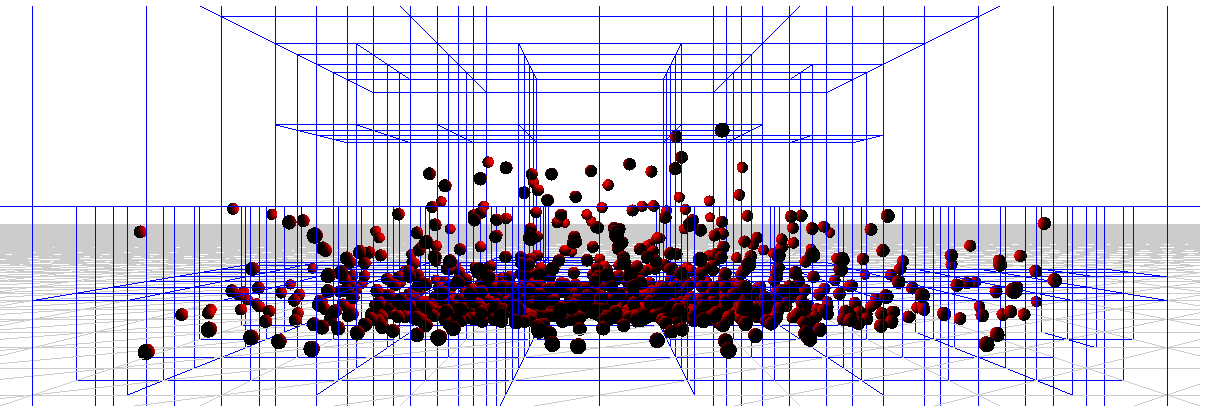
\includegraphics[width=16cm]{spheres/render2.png}
\end{figure}

Tests with Octree partitioning were executed with N=1000 spheres and T=1000 frames. The varying value is the maximum depth of Octree, ranging from 1 to 10.
Changing the maximum depth reduces the number of collision checks between spheres, as shown on \ref{img:octree-collisions}.

\begin{figure}[h!]
  \caption{Number of collisions in Octree}
  \label{img:octree-collisions}
  \centering
	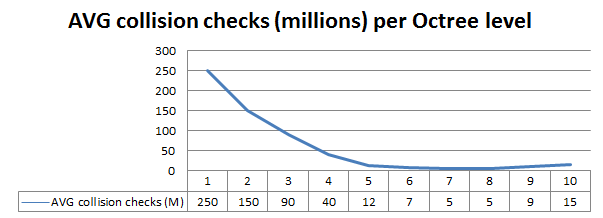
\includegraphics[width=16cm]{spheres/octree-collisions.png}
\end{figure}

For low values, the overall complexity of checks does not change significantly, since most spheres are in one or a few bounding cubes, and no checks are skipped. Additional operations related to Octree actually make this solution slower than $O(n^2)$ approach. For depth values in the optimal zone, the number of collisions is reduced by a factor of at least 10, while keeping Octree overhead reasonable. Interesting thing happens when the maximum level of Octree is very high and the edge of the smallest Octree cube approaches the size of the spheres. The number of transitions between partitioning cubes, related memory allocation and cleanups actually make this approach much slower, as shown on \ref{img:octree-time}. Moreover, some spheres are references in more than one cube, raising again the number of collision checks.

\begin{figure}[h!]
  \caption{Run times in Octree system}
  \label{img:octree-time}
  \centering
	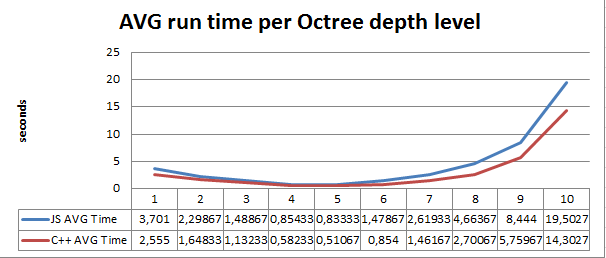
\includegraphics[width=16cm]{spheres/octree-time.png}
\end{figure}

It's clearly visible that the number of collision checks and run time is correlated only up to a certain point. For deep Octrees, the number of checks does not improve further, but the overall run time gets longer. The performance of JavaScript in relation to C++ varies between 30\% to 80\% overhead. In comparison with $O(n^2)$ approach, optimal Octree in JavaScript runs over 92\% faster and C++ over 94\% faster.
